\documentclass[tikz,border=7pt]{standalone}
\usetikzlibrary{angles,quotes,calc}
\begin{document}
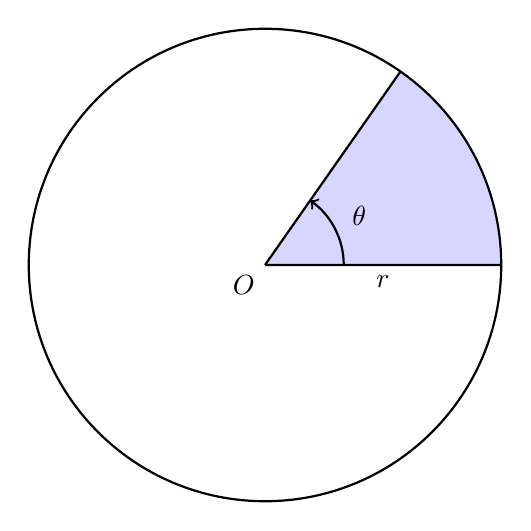
\begin{tikzpicture}[line width=.8pt]
\coordinate (O) at (0,0); \coordinate (A) at (3,0); \coordinate (B) at (55:3);
\fill[blue!16] (O)--(A) arc[start angle=0,end angle=55,radius=3]--cycle;
\draw (O) circle (3); \draw (O)--(A) (O)--(B);
\pic[draw,->,"$\theta$",angle radius=1cm,angle eccentricity=1.35] {angle=A--O--B};
\node[below left] at (O) {$O$}; \node[below] at ($(O)!.5!(A)$) {$r$};
\end{tikzpicture}
\end{document}
